\documentclass[tikz,border=4pt]{standalone}
% Shared style for every figure and for the deck: one accent, one
% highlight, thin lines, rounded nodes, nothing decorative.
\usepackage[T1]{fontenc}
\usepackage{lmodern}
\renewcommand{\familydefault}{\sfdefault}
\usepackage{tikz}
\usetikzlibrary{arrows.meta,positioning,calc,shapes.misc,fit,backgrounds,decorations.pathreplacing}
\definecolor{ink}{RGB}{40,40,40}
\definecolor{soft}{RGB}{150,150,150}
\definecolor{faint}{RGB}{225,225,225}
\definecolor{accent}{RGB}{0,95,115}
\definecolor{accentlight}{RGB}{214,232,236}
\definecolor{warn}{RGB}{196,84,40}
\definecolor{warnlight}{RGB}{247,226,216}
\tikzset{
  every picture/.style={color=ink, line width=0.5pt, font=\small},
  node distance=12mm and 18mm,
  box/.style={draw=ink, rounded corners=2pt, fill=white, inner sep=5pt, minimum height=7mm, align=center},
  maker/.style={box, minimum width=18mm},
  cat/.style={box, inner sep=3.5pt, minimum height=6mm},
  root/.style={box, fill=accentlight, draw=accent},
  bad/.style={box, fill=warnlight, draw=warn},
  ghost/.style={box, draw=soft, text=soft, dashed},
  flow/.style={-{Stealth[length=4pt,width=3.5pt]}, line width=0.5pt},
  sub/.style={-{Stealth[length=4pt,width=3.5pt]}, line width=0.5pt, color=soft},
  strong/.style={flow, color=accent, line width=0.8pt},
  wrong/.style={flow, color=warn},
  lbl/.style={font=\footnotesize, text=ink, inner sep=1.5pt, fill=white},
  note/.style={font=\footnotesize, text=soft, align=center},
  rate/.style={font=\footnotesize, text=accent, inner sep=1pt, fill=white},
}

\usepackage{amsmath}
\usepackage{pgfplots}
\pgfplotsset{compat=1.17}

\begin{document}
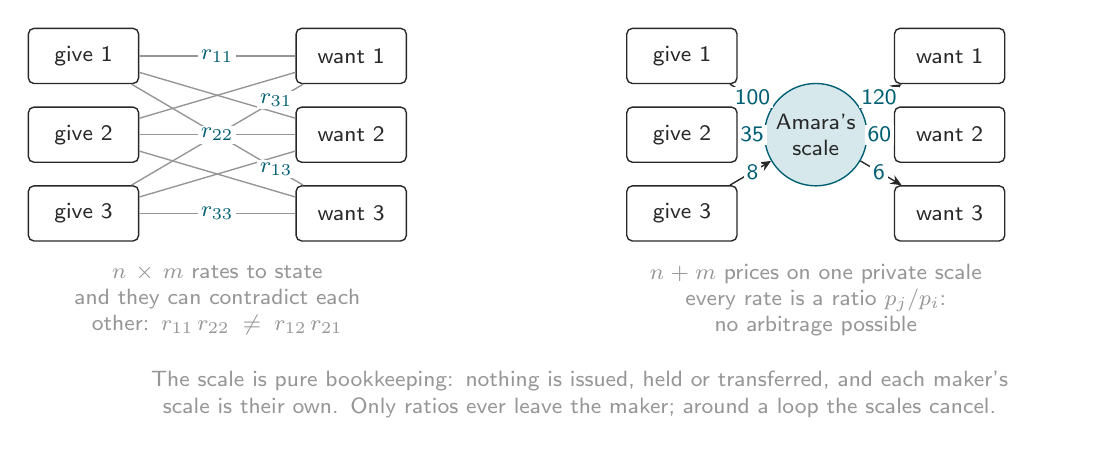
\begin{tikzpicture}[item/.style={box, inner sep=3pt, minimum width=14mm, font=\footnotesize}]
  % Left: every give against every want, n x m rates, mutually inconsistent
  % in general. Right: one private scale per maker, n + m prices, every
  % implied rate a ratio -- arbitrage-free by construction.
  \begin{scope}
    \foreach \i/\y in {1/10,2/0,3/-10} { \node[item] (g\i) at (0,\y mm) {give \i}; }
    \foreach \j/\y in {1/10,2/0,3/-10} { \node[item] (w\j) at (34mm,\y mm) {want \j}; }
    \foreach \i in {1,2,3} \foreach \j in {1,2,3} { \draw[soft] (g\i) -- (w\j); }
    \foreach \i/\j/\p in {1/1/0.5,2/2/0.5,3/3/0.5} { \node[rate] at ($(g\i)!\p!(w\j)$) {$r_{\i\j}$}; }
    \node[rate] at ($(g1)!0.72!(w3)$) {$r_{13}$};
    \node[rate] at ($(g3)!0.72!(w1)$) {$r_{31}$};
    \node[note, text width=44mm] at (17mm,-21mm) {$n \times m$ rates to state\\ and they can contradict each other: $r_{11}\,r_{22} \neq r_{12}\,r_{21}$};
  \end{scope}
  \begin{scope}[xshift=76mm]
    \node[root, circle, inner sep=1pt, minimum size=13mm, font=\footnotesize, align=center] (S) at (17mm,0) {Amara's\\ scale};
    \foreach \i/\y/\p in {1/10/100,2/0/35,3/-10/8} { \node[item] (g\i) at (0,\y mm) {give \i}; \draw[flow] (g\i) -- node[rate, pos=0.55] {\p} (S); }
    \foreach \j/\y/\p in {1/10/120,2/0/60,3/-10/6} { \node[item] (w\j) at (34mm,\y mm) {want \j}; \draw[flow] (S) -- node[rate, pos=0.45] {\p} (w\j); }
    \node[note, text width=48mm] at (17mm,-21mm) {$n + m$ prices on one private scale\\ every rate is a ratio $p_j/p_i$: no arbitrage possible};
  \end{scope}
  \node[note, text width=124mm] at (63mm,-33mm) {The scale is pure bookkeeping: nothing is issued, held or transferred, and each maker's scale is their own. Only ratios ever leave the maker; around a loop the scales cancel.};
\end{tikzpicture}
\end{document}
